\section{Implementation}
 \label{sec:nfvactor-implementation}

\begin{figure}[!h]
\begin{subfigure}[t]{0.49\linewidth}
   \centering
   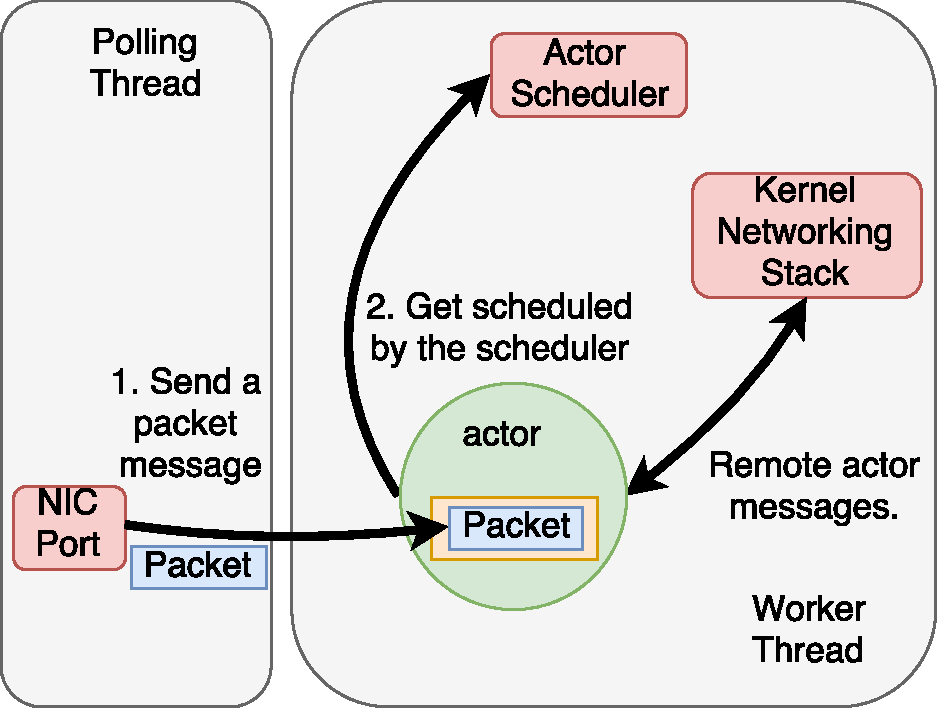
\includegraphics[width=\columnwidth]{chap-nfvactor/figure/actor-scheduling.pdf}
   \caption{Libcaf runtime.}\label{fig:actor-schedule}
  \end{subfigure}
  \begin{subfigure}[t]{0.49\linewidth}
     \centering
     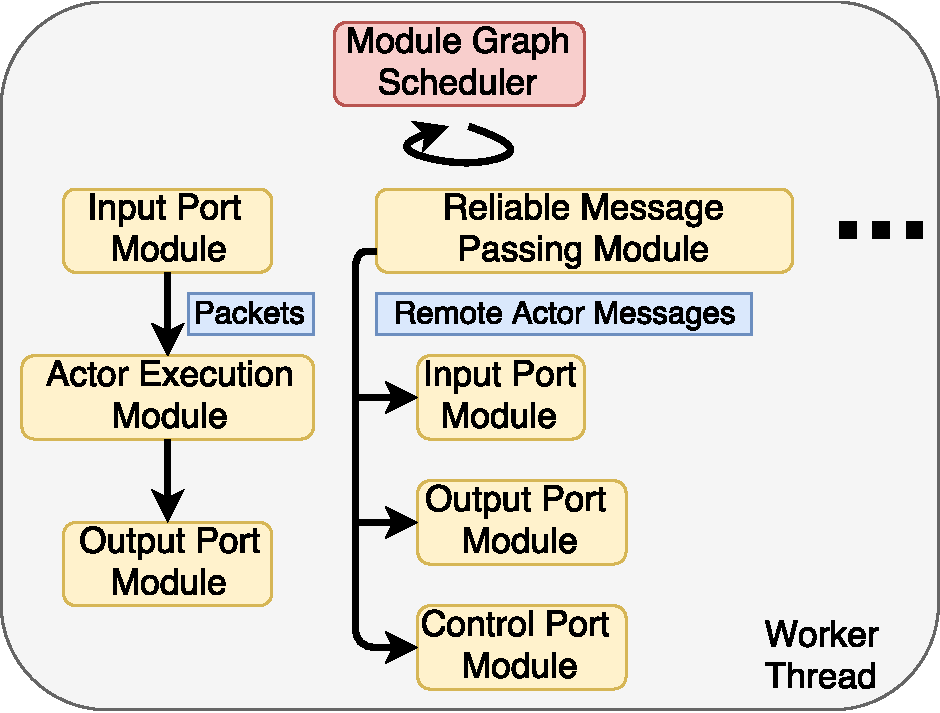
\includegraphics[width=\columnwidth]{chap-nfvactor/figure/graph-scheduling.pdf}
     \caption{\nfactor~runtime.}\label{fig:graph-schedule}
    \end{subfigure}
 \caption{Comparison of runtime architecture.}
\label{fig:two-versions}
\end{figure}

Throughout the development process of~\nfactor, we initially chose libcaf \cite{caf} as the runtime, whose architecture is shown in Fig.~\ref{fig:actor-schedule}. However, the performance of libcaf \cite{caf} runtime is less than satisfactory, for both packet processing and resilience operations. We believe that the performance problems of libcaf runtime come from two aspects. \textit{First}, the actor scheduler of libcaf is not suitable for handling IO of raw network packets. According to Fig.~\ref{fig:actor-schedule}, the scheduler schedules an actor run according to whether the actor has received a message. To inject dataplane packets into libcaf runtime, we have to set up a dedicated polling thread to poll the NIC port and send received packets to actors running in another worker thread by enqueueing the packet into actor's message queue. As verified in Sec.~\ref{sec:packet-processing-tl}, there is an expensive synchronization overhead between polling thread and worker thread, which may decrease packet processing throughput by over 100\%. \textit{Second}, libcaf runtime still relies on inefficient kernel networking thread to exchange remote actor messages with other runtimes.

Realizing these problems, we design a customized actor runtime for \nfactor~as shown in Fig.~\ref{fig:graph-schedule}, by leveraging two optimizations. \textit{First}, we implement a module graph scheduler to schedule actors according to several pre-defined module graphs. The module graph scheduler combines various IO operations (polling NIC port, exchanging remote actor messages) with actor scheduling inside a single worker thread, effectively eliminating the thread synchronization overhead as in libcaf. \textit{Second}, we bypass inefficient kernel networking stack and implement a high-performance, reliable message passing module running in user-space.

The tradeoff point when designing the customized runtime is programmability, as the programming interface exposed by the customized runtime is not as easy to use as the libcaf runtime. However, we believe that such a tradeoff is worthwhile due to improved performance.

% The~\nfactor~is implemented by about 8500 lines of code in C++, except the code for NFs. The implementation of \nfactor~has gone through a few trials and errors. Initially, we used libcaf \cite{caf} and implemented a runtime as shown in Fig.~\ref{fig:actor-schedule}. Even though libcaf is probably the fastest existing actor library \cite{chs-rapc-16}, performance of the first version is less than satisfactory, primarily due to the inefficacy of message passing through concurrent message queue and relying on kernel network stack for remote actor message transmission. The problems motivated us to design a customized actor library for \nfactor~and implement a new runtime as shown in Fig.~\ref{fig:graph-schedule}.

%\vspace{-2mm}
%\subsection{Customized Actor Library}

%We adopt three optimization strategies in our actor library to speed up packet processing. First, concurrent message queue is removed from each actor and message passing is transformed into direct function call. Second, in libcaf, an actor is scheduled to run after a message is placed into its message queue. Due to the first optimization, our library cannot follow libcaf's scheduling strategy. Instead, we implement a module graph scheduler to schedule actors according to several pre-defined module graphs (Sec.~\ref{sec:mgs}). Third, we bypass the kernel network stack and implement a reliable message passing module (Sec.~\ref{sec:rmp}) running in user-space.

\noindent \textbf{Module Graph Scheduler.} Inspired by the scheduler design of BESS \cite{bess} and Click \cite{kohler2000click}, the module graph scheduler keeps scheduling several module graphs to run in a round-robin fashion. A module graph consists of several processing modules, connected together into an acyclic graph. Inside a module graph, the actor messages are generated by a source module, flow through the connected module for processing before reaching the sink module, which consumes each message by either freeing it or sending it to the outside. Inside a module, the message handler of the corresponding actor is called for each actor message. The actor then pushes the processed message to the next connected module. When all the generated actor messages are consumed, the scheduler moves on to run the next module graph. % The module graph can be implemented as a function call graph, fulfilling our goal of removing actor queues.

Fig.~\ref{fig:graph-schedule} illustrates two module graphs. The first module graph polls dataplane packets from the input port and generates packet messages, which are pushed along the module graph, processed by the flow actors and sent out from the output port. The second module graph fetches remote actor messages from the reliable message passing module and sends the remote actor message out from one of the three ports. There are two other module graphs that are used for receiving reliable actor messages and interacting with the RPC requests.

% The idea of module graph was originally introduced in the Click modular router \cite{kohler2000click} and then extended by BESS \cite{bess}. However, we are the first to apply module graph scheduling to speed up actor processing.

%Remote actor messages passed among different runtimes should be reliably delivered.
\noindent \textbf{Reliable Message Passing.} Based on the module graph scheduler, we build a reliable message passing module, which inserts remote actor messages into a reliable packet stream for transmission. The module creates one ring buffer for each remote runtime and virtual switch. When a flow actor on this runtime sends a remote actor message, the module creates a packet, copies the content of the message into the packet and then enqueues the packet into the respective ring buffer. These packets are configured with a sequential number each, and appended with a special header to differentiate them from dataplane packets. When the second module graph in Fig.~\ref{fig:graph-schedule} is scheduled to run, the worker thread dequeues these packets from the ring buffers, and sends them to respective remote runtimes. A remote runtime acknowledges receipt of such packets. Retransmission is fired in case that the acknowledgement for a packet is not received after a configurable timeout (\eg, 10 times the RTT in our current implementation). Running entirely in user-space, the performance of the reliable message passing module is good enough to saturate a 10Gbps link (Sec.~\ref{sec:srram}).

Since our goal is to reliably transmit remote actor messages over an inter-connected L2 network, we do not use user-level TCP \cite{jeong2014mtcp}, which may impose additional overhead for reconstructing byte streams into messages. In addition, packet-based reliable message passing provides additional benefits during flow migration and replication. Because the response in 2nd request-response step of flow migration is sent as a packet using the same path as the dataplane packets, reliable actor message passing enables us to implement loss-avoidance migration with ease (Sec.~\ref{sec:migration}).



%Since our goal is to reliably transmit remote actor messages over an inter-connected L2 network, we do not use user-level TCP \cite{jeong2014mtcp}, which may impose much more processing overhead for reconstructing byte streams into messages. %In addition, packet-based reliable message passing provides additional benefits during flow migration and replication. Because the response in 2nd request-response step of flow migration is sent as a packet using the same path as the dataplane packets, reliable actor message passing enables us to implement loss-avoidance migration with ease (Sec.~\ref{sec:migration}).
